\documentclass[aspectratio=169]{beamer}
\usepackage{will_handley_beamer}
\usepackage{title_page}
\usepackage{slashed}
\usetikzlibrary{positioning}
\usetikzlibrary{calc}
\usetikzlibrary{fit}
\usepackage[percent]{overpic}

% Commands
% --------
% - \arxiv{arxiv number}
% - \arxiv{<number>}            arxiv.org/abs/<number>
% - \oldarxiv{<arxiv number>}   arxiv.org/<number>
% - \doi{<doi>}                 doi.org/<doi>
% - \xkcd{<number>}             xkcd.com/<number>
% - \email{<email>}             <<email>>
% - \tthref{<website>}          <website>
% - \av[dist]{<quantity>}       <quantity>_{dist}

% Talk details
% ------------
\title{Nested sampling \& simulation-based inference}
\subtitle{Next-generation statistical inference tools}
\date{13\textsuperscript{th} November 2024}

\begin{document}
%The most relevant branches are: `remotes/origin/ras_sbi_2024`, `remotes/origin/lcdm_2023`, `remotes/origin/tools_2021`, `remotes/origin/cavendish_2024`, `remotes/origin/cosmoverse_2024`, and `remotes/origin/adelaide_2020`.  Some older branches like `remotes/origin/garching_2015` and `remotes/origin/edinburgh_2016` also have useful introductory material on Nested Sampling, but the figures and explanations may be slightly outdated.
% Also phystat_2024 and phystat_imperial_2024


\begin{frame}
    \titlepage
\end{frame}

% remotes/origin/ras_sbi_2024
\begin{frame}
    \frametitle{Bayesian inference}
    \begin{itemize}
        \item A ``generative'' model $M$, with tunable parameters $\theta$, describing (compressed) data $D$.
            \begin{itemize}
                \item e.g. $M=\Lambda$CDM, $\theta=\{\Omega_b,\Omega_c, \tau, H_0, A_s, n_s\}$, $D=\{C_\ell\}$.
            \end{itemize}
        \item Described by simulation process $\theta\to D$, or likelihood $P(D|\theta,M)$.
        \item Frequentists \& Bayesians agree on the likelihood.
        \item Bayesians treat parameter space $\theta$ the same as data space $D$.
        \item Quantifying uncertainty with probability using Bayes theorem:
        \[
            \C[0]{P}(\theta|D,M) = \frac{\C[2]{P}(D|\theta,M)\C[1]{P}(\theta|M)}{\C[3]{P}(D|M)}, \quad \C[0]{\text{Posterior}} = \frac{\C[2]{\text{Likelihood}}\times\C[1]{\text{Prior}}}{\C[3]{\text{Evidence}}}.
        \]
    \end{itemize}
\end{frame}

% remotes/origin/ras_sbi_2024
\begin{frame}
    \frametitle{The three pillars of Bayesian inference}
    \begin{description}
        \item[Parameter estimation] Given a model, which range of parameters best describe the data?
            \[ \C[0]{P(\theta|D,M)} = \frac{\C[2]{P(D|\theta,M)} \C[1]{P(\theta|M)}}{\C[3]{P(D|M)}}, \] 
            \[ \C[0]{\mathcal{P}} = \frac{\C[2]{\mathcal{L}} \times\C[1]{\pi}}{\C[3]{\mathcal{Z}}}, \] 
            \[ \C[0]{\text{Posterior}} = \frac{\C[2]{\text{Likelihood}} \times\C[1]{\text{Prior}}}{\C[3]{\text{Evidence}}}. \]
        \item[Model comparison] Which models do the data prefer?
            \[ \C[4]{P(M|D)} = \frac{\C[3]{P(D|M)} P(M)}{P(D)}, \] \[ \frac{\C[3]{\mathcal{Z}_\mathcal{M}} \Pi_\mathcal{M}}{\sum_m Z_m \Pi_m}, \] \[ \C[4]{\text{Posterior}} = \frac{\C[3]{\text{Evidence}} \times\text{Prior}}{\text{Normalisation}}.\]
        \item[Tension quantification] Are different (sub)sets of data consistent with one another?
            \[ \mathcal{R} = \frac{\C[3]{\mathcal{Z}}_{AB}}{\C[3]{\mathcal{Z}}_A\C[3]{\mathcal{Z}}_\mathcal{B}}, \] 
            \[
                \begin{aligned} \log\mathcal{S} = \av[{\C[0]{\mathcal{P}}_{AB}}]{\C[2]{\log\mathcal{L}}_{AB}}&\\
                    -\av[{\C[0]{\mathcal{P}}_{A}}]{\C[2]{\log\mathcal{L}}_{A}}&\\
                    -\av[{\C[0]{\mathcal{P}}_{B}}]{\C[2]{\log\mathcal{L}}_{B}}&
                \end{aligned}
            \]
    \end{description}
\end{frame}

% remotes/origin/tools_2021
\begin{frame}
    \frametitle{Metropolis Hastings (baseline sampling algorithm)} 
    \begin{itemize}
        \item Turn the $N$-dimensional problem into a one-dimensional one.
        \item Pick start point $\theta_0$.
        \item At step $i$:
            \begin{enumerate}
                \item Propose a new point $\theta_{i+1}$ a small step away from $\theta_{i}$
                \item If uphill $\mathcal{P}(\theta_{i+1}) > \mathcal{P}(\theta_i)$, make step\ldots
                \item \ldots otherwise make step with probability $\alpha = \mathcal{P}(\theta_{i+1}) / \mathcal{P}(\theta_i)$. 
            \end{enumerate}
        \item Requires a proposal distribution $\mathcal{Q}(\theta_{i+1}|\theta_i)$
        \item In general case where $\mathcal{Q}$ is not symmetric, need acceptance ratio:
            \begin{equation*}
                \alpha = \frac{\mathcal{P}(\theta_{i+1})\mathcal{Q}(\theta_{i}|\theta_{i+1})}{\mathcal{P}(\theta_{i})\mathcal{Q}(\theta_{i+1}|\theta_{i})}
            \end{equation*}
    \end{itemize}
\end{frame}

% remotes/origin/tools_2021
\begin{frame}
    \frametitle{Nested sampling (high dimensional integration)}
    \begin{columns}
        \column{0.5\textwidth}
        \begin{itemize}
            \item Start with $n$ random samples over the space.
            \item Delete outermost sample, and replace with a new random one at higher integrand value.
            \item The ``live points'' steadily contract around the peak(s) of the function.
            \item We can use this evolution to estimate volume \emph{probabilistically}.
            \item At each iteration, the contours contract by $\sim\frac{1}{n}\only<9->{\pm \frac{1}{n}}$ of their volume.
            \item This is an exponential contraction, so
                \[  \sum_i f(x_i) \Delta V_i, \qquad V_i = V_0 e^{-\only<9->{(}i\only<9->{\pm\sqrt{i})}/n} \]
        \end{itemize}
        \column{0.5\textwidth}
        \includegraphics<1|handout:0>[width=\textwidth,page=1]{figures/himmelblau}%
        \includegraphics<2|handout:0>[width=\textwidth,page=2]{figures/himmelblau}%
        \includegraphics<3|handout:0>[width=\textwidth,page=3]{figures/himmelblau}%
        \includegraphics<4          >[width=\textwidth,page=4]{figures/himmelblau}%
        \includegraphics<5|handout:0>[width=\textwidth,page=5]{figures/himmelblau}%
        \includegraphics<6|handout:0>[width=\textwidth,page=6]{figures/himmelblau}%
        \includegraphics<7|handout:0>[width=\textwidth,page=7]{figures/himmelblau}%
        \includegraphics<8-|handout:0>[width=\textwidth,page=8]{figures/himmelblau}%
    \end{columns}
\end{frame}

% remotes/origin/tools_2021
\begin{frame}
    \frametitle{The nested sampling meta-algorithm}
    \begin{columns}
        \column{0.5\textwidth}
        \begin{itemize}
            \item At the end, one is left with a set of discarded ``dead'' points.
            \item Nested sampling estimates the \textbf{density of states} and calculates partition functions
                \[Z(\beta) = \sum_i f(x_i)^\beta \Delta V_i\]
            \item The evolving ensemble of live points allows:
                \begin{itemize}
                    \item implementations to self-tune
                    \item exploration of multimodal functions
                    \item global and local optimisation
                \end{itemize}
            \item For this kind of numerical, generic, high-dimensional integration, it is the only game in town.
        \end{itemize}
        \column{0.5\textwidth}
        \includegraphics[width=\textwidth,page=14]{figures/himmelblau}%
    \end{columns}
\end{frame}


% remotes/origin/ras_sbi_2024
\begin{frame}
    \frametitle{Simulation-based inference}
    \begin{columns}
        \column{0.5\textwidth}
        \begin{itemize}
            \item Only have access to a forward model $\theta \rightarrow D$.
            \item $(\theta,D)$ plane gives a more expansive theoretical view of inference.
            \item Forward model defines \emph{implicit} likelihood~$\mathcal{L}$:
            \item Simulator generates samples from $\mathcal{L}(D|\theta)$.
            \item With a prior $\pi(\theta)$ can generate samples from joint distribution~$\mathcal{J}(\theta,D)=\mathcal{L}(D|\theta)\pi(\theta)$\\\hfill \emph{the ``probability of everything''}.
            \item Task of SBI is then to go from joint~$\mathcal{J}$ to posterior $\mathcal{P}(\theta|D)$ and evidence $\mathcal{Z}(D)$ -- and possibly likelihood $\mathcal{L}(D|\theta)$.
            \item SBI \& forward modelling force us to think about data space~$D$ \& parameter space~$\theta$.
        \end{itemize}
        \column{0.5\textwidth}
        \includegraphics<1->[page=21, width=\textwidth]{figures/sbi_parameter_estimation.pdf}%
    \end{columns}
\end{frame}


% remotes/origin/ras_sbi_2024
\begin{frame}
    \frametitle{Neural Ratio Estimation}
    \begin{columns}
        \column{0.5\textwidth}
        \begin{itemize}
            \item SBI flavours:
                {\small
                    \begin{description}
                        \item[NPE] Neural posterior estimation
                        \item[NLE] Neural likelihood estimation
                        \item[NJE] Neural joint estimation
                        \item[NRE] Neural ratio estimation
                    \end{description}
                }
            \item NRE recap:
                \begin{enumerate}
                    \item Generate joint samples $(\theta,D)\sim\mathcal{J}$
                        \begin{itemize}
                            \item \textit{straightforward if you have a simulator:\\ $\theta\sim\pi(\cdot)$, $D\sim\mathcal{L}(\cdot|\theta)$}
                        \end{itemize}
                    \item Generate separated samples $\theta\sim\pi$, $D\sim\mathcal{Z}$
                        \begin{itemize}
                            \item \textit{aside: can shortcut by scrambling the $(\theta,D)$ pairings}
                        \end{itemize}
                    \item Train probabilistic classifier $p$ to distinguish whether $(\theta,D)$ came from $\mathcal{J}$ or $\pi\times\mathcal{Z}$.
                    \item $\frac{p}{1-p} = r = \frac{P(\theta,D)}{P(\theta)P(D)} 
                        =
                        \frac{\mathcal{J}}{\pi\times\mathcal{Z}} = \frac{\mathcal{L}}{\mathcal{Z}} = \frac{\mathcal{P}}{\pi}$.
                    \item Use ratio $r$ for parameter estimation $\mathcal{P} = r\times\pi$
                \end{enumerate}
        \end{itemize}
        \column{0.5\textwidth}
        \only<1|handout:0>{
            \begin{tikzpicture}[node distance=1cm, every neuron/.style={circle, draw, minimum size=1cm},]
                \node[every neuron/.try] (j2)  {};
                \node[every neuron/.try, above left = 0cm and 0.5cm of j2] (theta) { $\theta$};
                \node[every neuron/.try, below left = 0cm and 0.5cm of j2] (D) { $D$};
                \node[every neuron/.try, above = 0.5cm of j2] (j1) {};
                \node[every neuron/.try, below = 0.5cm of j2] (j3) {};
                \node[every neuron/.try, above right = 0cm and 0.5cm of j2] (h1) {};
                \node[every neuron/.try, below right = 0cm and 0.5cm of j2] (h2) {};
                \node[every neuron/.try, right = 1.3cm of j2] (p) { $p$};
                \node[every neuron/.try, right = 0.5cm of p] (logr) { $r$};
                \draw[-] (theta) -- (j1);
                \draw[-] (D) -- (j1);
                \draw[-] (theta) -- (j2);
                \draw[-] (D) -- (j2);
                \draw[-] (theta) -- (j3);
                \draw[-] (D) -- (j3);
                \draw[-] (j1) -- (h1);
                \draw[-] (j1) -- (h2);
                \draw[-] (j2) -- (h1);
                \draw[-] (j2) -- (h2);
                \draw[-] (j3) -- (h1);
                \draw[-] (j3) -- (h2);
                \draw[-] (h1) -- (p);
                \draw[-] (h2) -- (p);
                \draw[-] (p) -- (logr);
                \node[below =0.5cm of logr] {\includegraphics[page=22, width=0.5\textwidth]{figures/sbi_parameter_estimation.pdf}};
            \end{tikzpicture}
        }
    \end{columns}
\end{frame}

% remotes/origin/ras_sbi_2024
\begin{frame}
    \frametitle{TMNRE: Truncated Marginal Neural Ratio Estimation}
    \framesubtitle{\texttt{swyft}: \tthref{github.com/undark-lab/swyft}}
    \begin{columns}
        \column{0.55\textwidth}
        \begin{itemize}
            \item Two tricks for practical NRE:
        \end{itemize}
        \begin{block}{Marginalisation}
            \begin{itemize}
                \item Only consider one or two parameters at a time.
                \item Fine if your goal is to produce triangle plots.
                \item Problematic if information is contained jointly in more than two parameters.
            \end{itemize}
        \end{block}
        \begin{block}{Truncation}
            \begin{itemize}
                \item focus parameters $\theta$ on a subset of the prior which reproduces observed data $D_\text{obs}$
                \item region is somewhat arbitrary (usually a box)
                \item not amortised, sounds a bit like ABC
            \end{itemize}
        \end{block}
        \column{0.45\textwidth}
        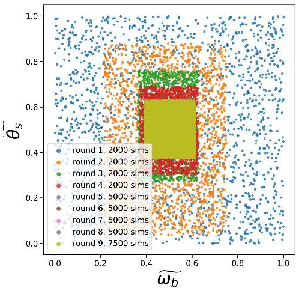
\includegraphics[width=\textwidth]{figures/tmnre}
    \end{columns}
\end{frame}

% remotes/origin/lcdm_2023
\begin{frame}
    \frametitle{Nuisance marginalised likelihoods: Theory \arxiv{2207.11457}}
    \begin{columns}[t]
        \column{0.5\textwidth}
        \begin{itemize}
            \item Bayes theorem
                \begin{align}
                    \C[2]{\mathcal{L}}(\theta,\alpha) 
                    \times 
                    \C[1]{\pi}(\theta,\alpha) &= 
                    \C[0]{\mathcal{P}}(\theta,\alpha)
                    \times
                    \C[3]{\mathcal{Z}}\\
                    \C[2]{\text{Likelihood}}
                    \times
                    \C[1]{\text{Prior}}
                    &=
                    \C[0]{\text{Posterior}}
                    \times
                    \C[3]{\text{Evidence}}
                    \nonumber
                \end{align}
                \small{$\alpha$: nuisance parameters, $\theta$: cosmo parameters.}
            \item Marginal Bayes theorem
                \begin{equation}
                    \C[2]{\mathcal{L}}(\theta) 
                    \times 
                    \C[1]{\pi}(\theta) = 
                    \C[0]{\mathcal{P}}(\theta)
                    \times
                    \C[3]{\mathcal{Z}}
                \end{equation}
            \item Non-trivially gives \textbf{nuisance-free likelihood}
                \begin{equation}
                    \boxed{
                        \C[2]{\mathcal{L}}(\theta) 
                        = 
                        \frac{
                            \C[0]{\mathcal{P}}(\theta)
                            \C[3]{\mathcal{Z}}
                        }{
                            \C[1]{\pi}(\theta)
                        }
                    }
                    =
                    \frac{
                        \int \C[2]{\mathcal{L}}(\theta,\alpha) \C[1]{\pi}(\theta,\alpha) d{\alpha}
                    }
                    {
                        \int \C[1]{\pi}(\theta,\alpha) d{\alpha}
                    }
                \end{equation}
        \end{itemize}
        \column{0.5\textwidth}
        \textbf{Key properties}
        \begin{itemize}
            \item Given datasets $A$ and $B$, each with own nuisance parameters $\alpha_A$ and $\alpha_B$:
            \item If you use $\mathcal{L}_A(\theta)$, you get the same (marginal) posterior and evidence if you had run with nuisance parameters $\alpha_A$ (ditto $B$).
            \item If you run inference on $\mathcal{L}_A(\theta)\times\mathcal{L}_B(\theta)$, you get the same (marginal) posterior and evidence if you had run with all nuisance parameters $\alpha_A$, $\alpha_B$ on.
            \item[] \textit{(weak marginal consistency requirements on joint $\pi(\theta,\alpha_A,\alpha_B)$ and marginal priors)}
        \end{itemize}
    \end{columns}
\end{frame}

% remotes/origin/lcdm_2023
\begin{frame}
    \frametitle{Nuisance marginalised likelihoods: Practice~{\small\arxiv{2205.12841}}}
    \begin{columns}
        \column{0.6\textwidth}
        \begin{columns}
            \column{0.3\textwidth}
            \[
                \boxed{
                    \C[2]{\mathcal{L}}(\theta) 
                    = 
                    \frac{
                        \C[0]{\mathcal{P}}(\theta)
                        \C[3]{\mathcal{Z}}
                    }{
                        \C[1]{\pi}(\theta)
                    }
                }
            \]
            \column{0.7\textwidth}
            \begin{itemize}
                \item To compute the nuisance marginalised likelihood, need:
                    \begin{enumerate}
                        \item Bayesian evidence $\C[3]{\mathcal{Z}}$
                        \item Marginal prior and posterior \textbf{densities}
                    \end{enumerate}
            \end{itemize}
        \end{columns}
        \begin{enumerate}
            \item Use nested sampling to compute evidence $\C[3]{\mathcal{Z}}$ and marginal samples $\{\theta,\alpha\}_\mathcal{P}$ and $\{\theta,\alpha\}_\pi$.
            \item Use normalising flows to compute density estimators $\C[0]{\mathcal{P}(\theta)}$, $\C[1]{\pi(\theta)}$ from marginal samples.
        \end{enumerate}
        \begin{itemize}
            \item Emulators usually much faster than original likelihoods
            \item \texttt{margarine}: PyPI, \href{https://github.com/htjb/margarine}{github.com/htjb/margarine}
        \end{itemize}

        \column{0.4\textwidth}
        \begin{tikzpicture}[
                rednode/.style={rectangle, draw=red!60, fill=red!5, very thick, minimum size=5mm},
                bluenode/.style={rectangle, draw=blue!60, fill=blue!5, very thick, minimum size=5mm},
                greennode/.style={rectangle, draw=green!60, very thick, minimum size=5mm},
                node distance=0.5cm,
                remember picture, overlay
            ]
            \node<1->[bluenode, xshift=0.5\textwidth, yshift=-0.25\textwidth](likelihood) at (current page.north)  {$ \mathcal{L}(\theta,\alpha)$};
            \node<1->[bluenode, right = of likelihood.east](prior) {$ \pi(\theta,\alpha)$};

            \coordinate<1-> (likelihoodprior) at ($(likelihood.south)!0.5!(prior.south)$);

            \node<2->[rednode, below = of likelihoodprior](nestedsampling) {Nested Sampling};
            \draw<2->[->](likelihood.south) -- (likelihood|-nestedsampling.north);
            \draw<2->[->](prior.south) -- (prior|-nestedsampling.north);

            \node<3->[bluenode, below = of nestedsampling](posterior) {$ \{\theta,\alpha\}_\mathcal{P}$};
            \draw<3->[->](nestedsampling.south-|posterior) -- (posterior.north);
            \node<4->[bluenode, left = of posterior.west](evidence) {$ \mathcal{Z}$};
            \draw<4->[->](nestedsampling.south-|likelihood) -- (evidence.north);
            \node<5->[bluenode, right = of posterior.east](priorSamples) {$ \{\theta,\alpha\}_\pi$};
            \draw<5->[->](nestedsampling.south-|prior) -- (priorSamples.north);

            \coordinate<5-> (posteriorprior) at ($(posterior.south)!0.5!(priorSamples.south)$);

            \node<6->[rednode, below = of posteriorprior](margarine)  {Density Estimation};

            \draw<6->[->](posterior.south) -- (margarine.north-|posterior.east);
            \draw<6->[->](priorSamples.south) -- (margarine.north-|priorSamples.west);

            \node<7->[bluenode, below = of posterior|-margarine.south](marginalPosterior) {$ \mathcal{P}(\theta)$};


            \draw<7->[->](margarine.south-|marginalPosterior.east) -- (marginalPosterior.north);


            \node<8->[bluenode, below = of marginalPosterior.south-|margarine.south-|priorSamples](marginalPrior) {$ \pi(\theta)$};
            \draw<8->[->](margarine.south-|priorSamples.west) -- (marginalPrior.north);


            \node<9->[bluenode, below = of marginalPosterior](marginalLikelihood) {$ \mathcal{L}(\theta)$};


            \draw<9->[->](evidence.south) -- (marginalLikelihood.west);
            \draw<9->[->](marginalPosterior.south) -- (marginalLikelihood.north);
            \draw<9->[->](marginalPrior.west) -- (marginalLikelihood.east);

            \node<10->[greennode,behind path,fit=(nestedsampling) (marginalPosterior) (priorSamples) (evidence),] {};

        \end{tikzpicture}
    \end{columns}
\end{frame}

\begin{frame}
    \frametitle{Jax-based nested samplers}
\end{frame}

\begin{frame}
    \frametitle{Accelerated nested sampling with beta flows}
\end{frame}


\begin{frame}
    \frametitle{Conclusions}
\end{frame}

\end{document}


\end{document}
